% Basado en el template realizado por Diego Essaya, disponible en
%                                                         http://lug.fi.uba.ar
% Modificado por Sebastián Santisi.
% 2007: Modificado por Patricio Moreno y Michel Peterson.
% 2014: Modificado por Patricio Moreno.
% 2017: Modificado por Patricio Moreno.
% 2021: Modificado por Carla Sobico.
% 2024: Modificado(simplificado) por Francisco Del Rio.

% Acá se define el tamaño de letra principal:
% Para utilizar los estilos de KOMA-script, desconectar la línea siguiente y
% comentar la que le sigue (dejar sin comentar un único documentclass)
%\documentclass[10pt, spanish]{scrartcl}
\documentclass[a4paper, twoside, 10pt, spanish]{article}

%%%%%%%%%%%%%%%%%%%%%%%%%%%%%%
% CS
%%%%%%%%%%%%%%%%%%%%%%%%%%%%%%
\usepackage{listings}

\usepackage{booktabs}
\usepackage[margin=1in]{geometry}
\usepackage{array}
\usepackage{pdflscape}
\usepackage{multirow}
\usepackage{float}

% CONFIGURACIONES GENERALES
%%%%%%%%%%%%%%%%%%%%%%%%%%%%%%%%%%%%%%%%%%%%%%%%%%%%%%%%%%%%%%%%%%%%%%%%%%%%%
% Definición del tamaño de página y los márgenes:
% Si preferís menos márgenes, descomentá la línea siguiente
%\usepackage[a4paper,headheight=16pt,scale={0.7,0.8},hoffset=0.5cm]{geometry}
\usepackage[demo]{graphicx}
\usepackage{caption}
\usepackage{subcaption}
\usepackage{babel}  % contiene la correcta separación en sílabas del español
\usepackage[utf8x]{inputenc}    % porque el encoding del documento es UTF-8
\usepackage[per-mode=fraction]{siunitx}
\sisetup%
{
	output-decimal-marker = {,},
	exponent-product = \cdot,
    group-digits = integer,
	group-separator = {.}
}


%
% El paquete amsmath agrega algunas funcionalidades extra a las fórmulas.
% Además defino la numeración de las tablas y figuras al estilo "Figura 2.3",
% en lugar de "Figura 7". (Por lo tanto, aunque no uses fórmulas, si querés
% este tipo de numeración dejá el paquete amsmath descomentado).
%
\usepackage{amsmath, amsfonts, amssymb}
%\numberwithin{equation}{section}
%\numberwithin{figure}{section}
\numberwithin{table}{section}
%%%%%%%%%%%%%%%%%%%%%%%%%%%%%%%%%%%%%%%%%%%%%%%%%%%%%%%%%%%%%%%%%%%%%%%%%%%%%

%%%%%%%%%%%%%%%%%%%%%%%%%%%%%%%%%%%%%%%%%%%%%%%%%%%%%%%%%%%%%%%%%%%%%%%%%%%%%
% ENCABEZADO y PIE DE PÁGINA
%%%%%%%%%%%%%%%%%%%%%%%%%%%%%%%%%%%%%%%%%%%%%%%%%%%%%%%%%%%%%%%%%%%%%%%%%%%%%
\usepackage{fancyhdr}   % Para poder personalizarlo
\usepackage{lastpage}   % Para poder saber cuántas páginas tiene el documento
\pagestyle{fancy}
\renewcommand{\sectionmark}[1]{\markboth{}{\thesection\ \ #1}}
\fancyhead{}	% Elimino el contenido del encabezado
% Muestra la sección a la derecha (izquierda) en páginas impares (pares)
\fancyhead[RO,LE]{\rightmark}
% El siguiente texto a la derecha (izquierda) en páginas pares (impares)
\fancyhead[RE,LO]{TA138 - Segundo checkpoint}
\fancyfoot{}	% Elimino el contenido del pie de página
% A la izquierda (derecha) en páginas pares (impares): nro. de página / total
\fancyfoot[LE,RO]{\thepage/\pageref{LastPage}}
%%%%%%%%%%%%%%%%%%%%%%%%%%%%%%%%%%%%%%%%%%%%%%%%%%%%%%%%%%%%%%%%%%%%%%%%%%%%%

%%%%%%%%%%%%%%%%%%%%%%%%%%%%%%%%%%%%%%%%%%%%%%%%%%%%%%%%%%%%%%%%%%%%%%%%%%%%%
% Hipervínculos (enlaces) en el documento (y modificación de atributos)
%%%%%%%%%%%%%%%%%%%%%%%%%%%%%%%%%%%%%%%%%%%%%%%%%%%%%%%%%%%%%%%%%%%%%%%%%%%%%
\usepackage{url}
\urlstyle{tt}
\usepackage[colorlinks=true,linkcolor=black, urlcolor=blue]{hyperref}
\hypersetup{
    breaklinks,
    baseurl       = http://,
    pdfborder     = 0 0 0,
    pdfpagemode   = UseNone,
    pdfstartpage  = 1,
    pdfcreator    = {Plantilla de informe de TP para \LaTeX{}},
    bookmarksopen = true,
    bookmarksdepth= 2,% to show sections and subsections
    pdfauthor     = {Apellido~1, Apellido~2, Apellido~3},
    pdftitle      = {-},
    pdfsubject    = {Informe},
    pdfkeywords   = {}%
    }
%%%%%%%%%%%%%%%%%%%%%%%%%%%%%%%%%%%%%%%%%%%%%%%%%%%%%%%%%%%%%%%%%%%%%%%%%%%%%

%%%%%%%%%%%%%%%%%%%%%%%%%%%%%%%%%%%%%%%%%%%%%%%%%%%%%%%%%%%%%%%%%%%%%%%%%%%%%
% LISTAS (para poder modificar los 'bullets' de las listas)
%%%%%%%%%%%%%%%%%%%%%%%%%%%%%%%%%%%%%%%%%%%%%%%%%%%%%%%%%%%%%%%%%%%%%%%%%%%%%
\usepackage{enumerate}
%%%%%%%%%%%%%%%%%%%%%%%%%%%%%%%%%%%%%%%%%%%%%%%%%%%%%%%%%%%%%%%%%%%%%%%%%%%%%

%%%%%%%%%%%%%%%%%%%%%%%%%%%%%%%%%%%%%%%%%%%%%%%%%%%%%%%%%%%%%%%%%%%%%%%%%%%%%
% TABLAS (para que se vean bien)
%%%%%%%%%%%%%%%%%%%%%%%%%%%%%%%%%%%%%%%%%%%%%%%%%%%%%%%%%%%%%%%%%%%%%%%%%%%%%
\usepackage{booktabs}
\usepackage{multirow}
%%%%%%%%%%%%%%%%%%%%%%%%%%%%%%%%%%%%%%%%%%%%%%%%%%%%%%%%%%%%%%%%%%%%%%%%%%%%%

%%%%%%%%%%%%%%%%%%%%%%%%%%%%%%%%%%%%%%%%%%%%%%%%%%%%%%%%%%%%%%%%%%%%%%%%%%%%%
% IMÁGENES
%%%%%%%%%%%%%%%%%%%%%%%%%%%%%%%%%%%%%%%%%%%%%%%%%%%%%%%%%%%%%%%%%%%%%%%%%%%%%
% Para incluir imágenes, el siguiente código carga el paquete graphicx
% según se esté generando un archivo dvi o un pdf (con pdflatex).

% Para generar dvi, descomentá la linea siguiente:
%\usepackage[dvips]{graphicx}

% Para generar pdf, descomentá las dos lineas seguientes:
\usepackage{graphicx}
\pdfcompresslevel=9

% Todas las imágenes están en el directorio imgs:
\newcommand{\imgdir}{imgs}
\graphicspath{{\imgdir/}}
%%%%%%%%%%%%%%%%%%%%%%%%%%%%%%%%%%%%%%%%%%%%%%%%%%%%%%%%%%%%%%%%%%%%%%%%%%%%%

%%%%%%%%%%%%%%%%%%%%%%%%%%%%%%%%%%%%%%%%%%%%%%%%%%%%%%%%%%%%%%%%%%%%%%%%%%%%%
% DIAGRAMAS DE FLUJO EN DIA
%%%%%%%%%%%%%%%%%%%%%%%%%%%%%%%%%%%%%%%%%%%%%%%%%%%%%%%%%%%%%%%%%%%%%%%%%%%%%
% Necesitas este paquete si haces los diagramas de flujo en el programa Dia
% y exportás a latex
%\usepackage{tikz}
%%%%%%%%%%%%%%%%%%%%%%%%%%%%%%%%%%%%%%%%%%%%%%%%%%%%%%%%%%%%%%%%%%%%%%%%%%%%%

%%%%%%%%%%%%%%%%%%%%%%%%%%%%%%%%%%%%%%%%%%%%%%%%%%%%%%%%%%%%%%%%%%%%%%%%%%%%%
% INSERCIÓN DE CÓDIGO FUENTE
%%%%%%%%%%%%%%%%%%%%%%%%%%%%%%%%%%%%%%%%%%%%%%%%%%%%%%%%%%%%%%%%%%%%%%%%%%%%%
% El paquete recomendado actualmente es minted.
% Documentación: https://www.ctan.org/pkg/minted
\usepackage[
        section,    % Numera el código según la sección
    ]{minted}
% minted provee los comandos:
% 1)  \mint[<opciones>]{<lenguaje>}<delimitador><código><delimitador>
% 2)  \mintinline[<opciones>]{<lenguaje>}<delimitador><código><delimitador>
% 3)  \inputminted[<opciones>]{<lenguaje>}{<archivo>}
\setminted[c]{
%        style=,
        linenos,            % Mostrar los números de línea
        numberfirstline,    % Numerar SIEMPRE la primera línea mostrada
        tabsize=4,          % Reemplazar las tabulaciones por 4 espacios
        autogobble          % Eliminar espacio sobrante al comienzo
    }
%%%%%%%%%%%%%%%%%%%%%%%%%%%%%%%%%%%%%%%%%%%%%%%%%%%%%%%%%%%%%%%%%%%%%%%%%%%%%
% COMANDOS UTILES
%%%%%%%%%%%%%%%%%%%%%%%%%%%%%%%%%%%%%%%%%%%%%%%%%%%%%%%%%%%%%%%%%%%%%%%%%%%%%
% los siguientes comandos permiten escribir de manera uniforme en todo el
% documento

% Para poder manejar los espacios al final de los comandos propios
\usepackage{xspace}

% Abreviatura de 'número' utilizando letras voladas (correcto español)
\newcommand{\Nro}{N.\textsuperscript{o}\xspace}
\newcommand{\nro}{n.\textsuperscript{o}\xspace}
%%%%%%%%%%%%%%%%%%%%%%%%%%%%%%%%%%%%%%%%%%%%%%%%%%%%%%%%%%%%%%%%%%%%%%%%%%%%%
% PAQUETES EXTRAS
%%%%%%%%%%%%%%%%%%%%%%%%%%%%%%%%%%%%%%%%%%%%%%%%%%%%%%%%%%%%%%%%%%%%%%%%%%%%%
\usepackage{circuitikz}
\usepackage{float}
\usepackage{multicol}
%\usepackage{pdfpages}
%\usepackage{subfigure}
%\usepackage{graphicx}%
\usepackage{gensymb}
%%%%%%%%%%%%%%%%%%%%%%%%%%%%%%%%%%%%%%%%%%%%%%%%%%%%%%%%%%%%%%%%%%%%%%%%%%%%%
%%%%%%%%%%%%%%%%%%%%%%%%%%%%%%%%%%%%%%%%%%%%%%%%%%%%%%%%%%%%%%%%%%%%%%%%%%%%%
% INICIO DEL DOCUMENTO
%%%%%%%%%%%%%%%%%%%%%%%%%%%%%%%%%%%%%%%%%%%%%%%%%%%%%%%%%%%%%%%%%%%%%%%%%%%%%
%%%%%%%%%%%%%%%%%%%%%%%%%%%%%%%%%%%%%%%%%%%%%%%%%%%%%%%%%%%%%%%%%%%%%%%%%%%%%
\begin{document}


%
% Carátula:
%
\begin{titlepage}

\thispagestyle{empty}

\begin{center}
\includegraphics[scale=0.3]{res/fiuba.pdf}\\
\large{\textsc{Universidad de Buenos Aires}}\\
\large{\textsc{Facultad de Ingeniería}}\\
% Modificar año y cuatrimestre
\small{Año 2025 - 2\textsuperscript{o} cuatrimestre}
\end{center}

\vfill

\begin{center} % Modificar el código de ser necesario
\Large{\underline{\textsc{Taller de diseño de circuitos electrónicos (TA138)}}}\\
\vspace{.5cm}
 \Large{\textsc{Cuarto checkpoint - Sistema de alimentación para aplicaciones industriales y automotrices}}
\end{center}

\vfill

 \begin{tabbing}

	\\\hspace{2cm}\=\+\\ \\
% %	FECHA : DD/MM/2019\\% \today\\
%TUTOR: Lorem ipsum dolor sit amet, \\
 \\
	ESTUDIANTES: Grupo 4\hspace{-1cm}\=\+\hspace{1cm}\=\hspace{6cm}\=\\
            Martin, Andrés	\>\> 110722\\ 
              \>\footnotesize{\verb!ammartin@fi.uba.ar!}\\
            Loñ, Julieta	\>\> 110663\\ 
              \>\footnotesize{\verb!jlon@fi.uba.ar!}\\ 		    
            Monti, Martina	\>\> 110574\\ 
              \>\footnotesize{\verb!mmonti@fi.uba.ar!}\\
            Del Rio, Francisco	\>\> 110761\\ 
              \>\footnotesize{\verb!fadelrio@fi.uba.ar!}\\           
 \end{tabbing}



\vfill

\hrule
\vspace{0.2cm}

% Modificar código de ser necesario
\noindent\small{TA138 - Taller de diseño de circuitos electrónicos \hfill}

\end{titlepage}

%
% Hago que las páginas se comiencen a contar a partir de aquí:
%
\setcounter{page}{1}

%
% Pongo el índice en una página aparte:
%

\tableofcontents
\newpage
%
% Inicio del TP:
%
\section{Introducción}

\quad En esta entrega se realizara el diseño de la fuente buck y el circuito PWM. Para la fuente buck se deben realizar los cálculos necesarios para obtener las características físicas del inductor que se utilizara para implementar dicho circuito.  

\quad Ambos circuitos se deben diseñar teniendo en cuenta las especificaciones requeridas por el trabajo. La eficiencia para la fuente buck y la frecuencia para el PWM.
%%%%%%%%%%%%%%%%%%%%%%%%%%%%%%%%%%%%%%%%%%%%%%%%%%%%%%%%%%%
\section{Fuente buck}
%%%%%%%%%%%%%%%%%%%%%%%%%%%%%%%%%%%%%%%%%%%%%%%%%%%%%%%%%%%
\subsection{Diseño y simulación}
\quad En las fuentes buck se busca reducir la tensión de entrada a un nivel inferior en la salida, manteniendo la alta eficiencia. Para ello se utilizan distintos componentes. Un MOSFET canal N (IRFZ44N) es utilizado para actuar como interruptor controlado por PWM (debido a este comportamiento de "llave", la tensión Drain-Source de este MOSFET es muy baja); el segundo NMOS (IRFZ44N) conduce la corriente cuando el primer transistor se encuentra apagado, implementando de esta manera las llaves ideales vistas en el circuito teórico. 

\quad También se agregan capacitores para evitar picos de tensión. El circuito cuenta además con un inductor, el cual almacena energía y suaviza la corriente. Este inductor debe calcularse con precisión para evitar sobrecalentamientos, tener tiempos de respuesta acordes y otros factores; es por esto que se le dedicará toda una sección a su diseño.

\quad Para obtener el valor de la inductancia primero se calculo el mínimo valor que puede tomar para que el circuito continúe funcionando de manera adecuada. Para eso se debió considerar el caso de mayor conmutación, en donde la resistencia de carga es máxima. 
\begin{equation*}
    R_{max} = \frac{V_o}{I_{s,min}} 
\end{equation*}
\quad Considerando que $V_o=9.5V$ y $I_{s,max} =$\SI{0.1}{\ampere} se obtiene $R_{max} = 95\ohm$. Luego, el inductor se calcula mediante la siguiente expresión.
\begin{equation}
    L_{cr} = \frac{(1-D)R_{max}}{2f}
\end{equation}
\quad Considerando que se va a tener un  $D_{min}$ y un $D_{max}$ dependiendo de la $V_{in}$ se calcularon ambos:
\begin{equation}
    D_{max} = \frac{V_o + V_{ds2}}{V_{in}-V_{ds1}+V_{ds2}} = \frac{9.5+0.049}{12} = 0.7957
\end{equation}
\begin{equation}
    D_{min} = \frac{V_o + V_{ds2}}{V_{in}-V_{ds1}+V_{ds2}} = \frac{9.5+0.049}{30} = 0.3183
\end{equation}
\quad Se calcularon dos valores de $L_{cr}$ y se utilizó el más alto de ambos que es el que cumple con lo pedido y presenta el peor caso para el inductor critico. 
\quad De las cuentas se obtuvo $L_{cr} =$\SI{250}{\micro\henry}. Sin embargo, se decidió utilizar un inductor L = \SI{300}{\micro\henry} para mayor seguridad y evitar que variaciones en el valor real del inductor presenten problemas graves en el circuito implementado.

\quad El valor del capacitor de salida se debe calcular considerando el ripple, por lo tanto el valor se calculo de manera iterativa. Se decidió un valor inicial de \SI{100}{\micro F} y se observo el valor del ripple con ese valor para luego poder aplicar la siguiente expresión:
\begin{equation}
    \Delta V_o = \frac{I_{L,max}-I_{L,min}}{8Cf}
\end{equation}
\quad Con un capacitor de \SI{47}{\micro F} se obtiene un $\Delta V_o = $\SI{2.5}{\milli V} que cumple con los requisitos de tension de salida.

\quad Una vez finalizado todo el desarrollo del circuito se consiguió el siguiente diseño.

\begin{figure}[H]
    \centering
    \includegraphics[width=\linewidth]{res/simulacion_buck.png}
    \caption{Circuito Fuente Buck}
    \label{fig:esquema_pwm}
\end{figure}

\quad La tensión de salida de la fuente buck:

\begin{figure}[H]
    \centering
    \includegraphics[width=\linewidth]{res/simu_vo_buck.png}
    \caption{Tension de salida de la fuente buck}
    \label{fig:vo_buck}
\end{figure}

\quad La corriente sobre el inductor:
\begin{figure}[H]
    \centering
    \includegraphics[width=\linewidth]{res/simu_il_buck.png}
    \caption{Corriente sobre el inductor}
    \label{fig:corriente_inductor}
\end{figure}

\quad En la \autoref{fig:vo_buck} se puede ver que, además de la oscilación, el valor medio no es constante, esto se atribuye a la necesidad de agrandar el error de convergencia admitido para asegurarse esta misma.
%%%%%%%%%%%%%%%%%%%%%%%%%%%%%%%%%%%%%%%%%%%%%%%%%%%%%%%%%%%
\subsection{Inductor}

\quad Al momento de diseñar el inductor se debieron tener en cuenta ciertos parámetros de funcionamiento de la fuente buck. La frecuencia trabajo es de \SI{130}{kHz}, la $I_{L_{max}} = 1.54 A $, la $I_{L_{min}} = 1.42 A$.

\quad Se obtuvieron las características físicas del inductor usando el método \textit{Tacca}. Se debe considerar $\sigma_{IL} \leq 5 \frac{A}{mm^2}$ para evitar el sobrecalentamiento del alambre. Considerando los núcleos disponibles comercialmente y la tabla de cables provista por \textit{Ericksson}, se realizaron los cálculos necesarios para obtener los siguientes parámetros.

\begin{table}[H]
\centering
\begin{tabular}{|c|c|}
\hline
\textbf{Parámetros} & \textbf{Valor} \\ \hline
Material del nucleo  & \textit{N87} \\ \hline
Nucleo &  EE3007\\ \hline
Cable de cobre &  AWG\#20\\ \hline
Inductancia [\micro Hy] & 300 \\ \hline
$l_g$ [mm]& 0.151 \\ \hline
Numero de vueltas & 25 \\ \hline
$\sigma_{IL} [\frac{A}{mm^2}]$ & 2.978 \\ \hline
$r_{Cu}$ [cm] & 0.0437 \\ \hline
$\delta$ [cm] & 0.021 \\ \hline
\end{tabular}
\caption{Especificaciones del inductor}
\label{tab:especif_inductor}
\end{table}
\quad Con los valores obtenidos no hay efecto pelicular. 

%%%%%%%%%%%%%%%%%%%%%%%%%%%%%%%%%%%%%%%%%%%%%%%%%%%%%%%%%%%
\subsection{Eficiencia}
\quad En los reguladores conmutados Buck una eficiencia ideal sería del $100\%$. Sin embargo, esta eficiencia resulta imposible en la realidad debido a perdidas por conmutación, resistencias parasitas, caídas en el MOSFET, entre otros factores. Debido a esto, la eficiencia real estará alrededor del $90\% - 95\%$. Esta eficiencia aumentará dependiendo de la optimización del PCB, un control preciso del ciclo de trabajo y un MOSFET acorde. 

\quad En el caso del circuito diseñado, al utilizar un MOSFET como reemplazo del diodo para la conmutación, se logra una reducción en la caída de tensión. Además, la elección del inductor y el capacitor logran una gran reducción en el ripple de corriente y tensión respectivamente, lo que mejora la eficiencia.

\quad La eficiencia del circuito se obtiene segun la siguiente expresión:
\begin{equation}
    eficiencia  = \frac{P_{salida}}{P_{entrada}}
\end{equation}
\begin{equation}
    \eta (9.3V)  = \frac{9.3*1.469}{24*0.00631} = 90.2\%
\end{equation}
\begin{equation}
      \eta(9.7V) = \frac{9.7*0.103}{24*0.045} = 91.5\%
\end{equation}
\quad Ambos resultados cumplen con la eficiencia pedida para ambas tensiones especificadas del regulador buck.
%%%%%%%%%%%%%%%%%%%%%%%%%%%%%%%%%%%%%%%%%%%%%%%%%%%%%%%%%%%
\subsection{Diseño de PCB}
\quad Para realizar el PCB de la fuente buck debió tenerse en cuenta el trazado de pistas. Aquí se tuvo en cuenta la separación entre ellas para así evitar capacitancias o inductancias parásitas. Además se debió mantener un cierto ancho de las pistas debido a la potencia que circula en ciertas zonas. Se planeó previamente el plano de masa para así mejorar el retorno de la corriente y reducir ruido. Teniendo todas estas cuestiones en consideración se obtuvo el siguiente diseño.

\begin{figure}[H]
    \centering
    \includegraphics[width=\linewidth]{res/pcb_buck.jpg}
    \caption{Diseño PCB frente Fuente Buck}
    \label{fig:esquema_pwm}
\end{figure}
\begin{figure}[H]
    \centering
    \includegraphics[width=\linewidth]{res/pcb_buck_dorso.jpg}
    \caption{Diseño PCB dorso Fuente Buck}
    \label{fig:esquema_pwm}
\end{figure}
%%%%%%%%%%%%%%%%%%%%%%%%%%%%%%%%%%%%%%%%%%%%%%%%%%%%%%%%%%%
\section{Circuito PWM}

\quad Como se mencionó antes, para la fuente buck se necesita una señal PWM que se ocupará de encender y apagar los MOSFETs. La forma de obtener tal señal utilizada es mediante la comparación de una señal triangular de \SI{130}{\kilo hz} con una tensión constante. La ventaja de obtener la señal PWM de esta forma es que la tensión constante que se compara con la señal triangular podrá ser una señal proporcional a el error de la tensión de salida con la tensión deseada, de esta forma cerrando el lazo y obteniendo una fuente buck a lazo cerrado.

%%%%%%%%%%%%%%%%%%%%%%%%%%%%%%%%%%%%%%%%%%%%%%%%%%%%%%%%%%%
\subsection{Diseño y simulación}

\quad La topología utilizada para obtener la señal deseada es la de la \autoref{fig:esquema_pwm}. Este circuito consta de un integrador con el operacional U3 y el capacitor, que recibe una señal cuadrada de la salida de U1, generando la triangular deseada, que luego se compara con V3 en U3, para finalmente tener la señal PWM deseada. Dado la alta frecuencia de oscilación utilizada, U1 y U3 son comparadores en vez de amplificadores operacionales.

\begin{figure}[H]
    \centering
    \includegraphics[width=\linewidth]{res/esquema_pwm.png}
    \caption{Circuito utilizado para generar la señal PWM}
    \label{fig:esquema_pwm}
\end{figure}

\quad Los valores utilizados para los resistores y capacitores son los presentados en la \autoref{tab:valores_comp_pwm}. Los mismos se obtuvieron de forma empírica, teniendo en cuenta la constante de tiempo $\tau = R3 \cdot C$.

\begin{table}[H]
\centering
\begin{tabular}{|c|c|}
\hline
\textbf{Componente} & \textbf{Valor} \\ \hline
R1 & \SI{100}{\kilo \ohm} \\ \hline
R2 & \SI{24}{\kilo \ohm} \\ \hline
R3 & \SI{2.7}{\kilo \ohm} \\ \hline
C & \SI{2.2}{nF} \\ \hline
\end{tabular}
\caption{Valores de los componentes del circuito PWM}
\label{tab:valores_comp_pwm}
\end{table}
\quad Al simular el circuito se obtuvieron las señales cuadrada y triangular de las figuras \ref{fig:simu_pwm_cuad} y \ref{fig:simu_pwm_triang}: 

\begin{figure}[H]
    \centering
    \includegraphics[width=\linewidth]{res/grafico_simu_pwm_cuad.png}
    \caption{Señal cuadrada simulada}
    \label{fig:simu_pwm_cuad}
\end{figure}

\begin{figure}[H]
    \centering
    \includegraphics[width=\linewidth]{res/grafico_simu_pwm_triang.png}
    \caption{Señal triangular simulada}
    \label{fig:simu_pwm_triang}
\end{figure}
%%%%%%%%%%%%%%%%%%%%%%%%%%%%%%%%%%%%%%%%%%%%%%%%%%%%%%%%%%%
\subsection{Diseño de PCB}

\begin{figure}[H]
    \centering
    \includegraphics[width=0.5\linewidth]{res/pcb_pwm.png}
    \caption{Circuito PCB PWM}
    \label{fig:pcb_pwm}
\end{figure}
\begin{figure}[H]
    \centering
    \includegraphics[width=0.5\linewidth]{res/pcb_pwm_frente.png}
    \caption{Circuito PCB PWM}
    \label{fig:pcb_pwm_frente}
\end{figure}
\quad Al momento de realizar el diseño del PCB se debieron tener en cuenta las consideraciones nombradas anteriormente. Ademas se tuvo presente que las pistas debían evitar recorridos de gran distancia ya que al transportar frecuencia si estas son muy largas se puede generar ruido en la información. 

\quad Se agregaron pines de prueba al circuito en lugares estratégicos para luego poder verificar el funcionamiento del circuito, pudiendo observar la señal en donde es necesario que cumplan con formas y frecuencias especificas. Por lo tanto los pines agregados son en tierra, en la salida del comparador y en la salida del integrador. 

\quad Ademas como los comparadores son \textit{open collector} se agregaron resistencias de pull up conectadas a su salida. Se eligió el valor teniendo en cuenta lo recomendado por la datasheet del modelo y buscando evitar que se limite la corriente. 

\begin{figure}[H]
    \centering
    \includegraphics[width=0.5\linewidth]{res/pwm_frente.jpeg}
    \caption{Circuito PWM}
    \label{fig:pwm_frente}
\end{figure}

\begin{figure}[H]
    \centering
    \includegraphics[width=0.5\linewidth]{res/pwm_frente.jpeg}
    \caption{Circuito PWM}
    \label{fig:esquema_pwm}
\end{figure}

\quad Durante la implementación se observo que el valor de capacitancia elegido inicialmente era muy cercano al del capacitor interno del operacional y por lo tanto se deformaba la señal. Para solucionarlo se cambio la relación del RC, se aumento el valor del capacitor y se disminuyo el de la resistencia.
%%%%%%%%%%%%%%%%%%%%%%%%%%%%%%%%%%%%%%%%%%%%%%%%%%%%%%%%%%
\subsection{Mediciones}
\quad Al llevar a cabo las mediciones, se observó la señal cuadrada generada por el circuito a una frecuencia aproximada de 130kHz, tal como fue diseñada. Esta señal presenta transiciones rápidas por lo que se garantiza una conmutación correcta y eficiente de los MOSFETs en la fuente Buck. La amplitud de la señal se mantiene estable en el tiempo, sin ningún tipo de distorsiones.

\quad Por otro lado, la señal triangular muestra una forma simétrica y estable con una amplitud adecuada. Se observó que la frecuencia de oscilación también es de aproximadamente 130KHz.

\quad Se puede observar una distorsión en la señal triangular que se genera debido a la integración del sobrepico en la señal cuadrada. 

\quad Las posibles causas de este sobrepico son el problema ya antes mencionado de las capacidades de entrada del operacional o interferencias causadas por ruido generado en las pistas del PCB. 

\quad A pesar de lo mencionado, estas mediciones se puede confirmar el correcto funcionamiento del PWM, asegurando así una señal de control para la fuente conmutada Buck estable cumpliendo todos los requisitos.
\begin{figure}[H]
    \centering
    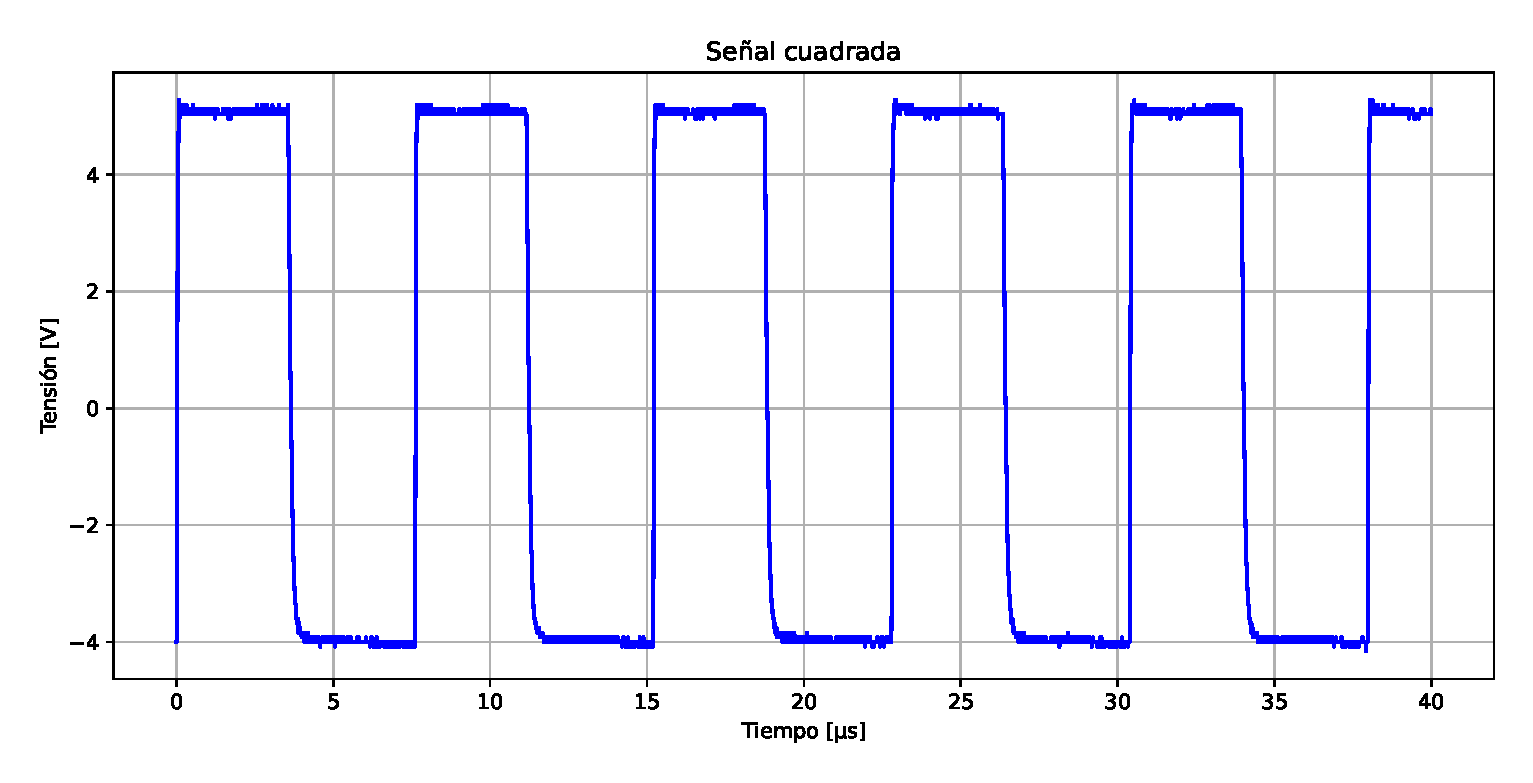
\includegraphics[width=\linewidth]{res/cuadrada.eps}
    \caption{Señal cuadrada}
    \label{fig:seña_cuadrada}
\end{figure}
\begin{figure}[H]
    \centering
    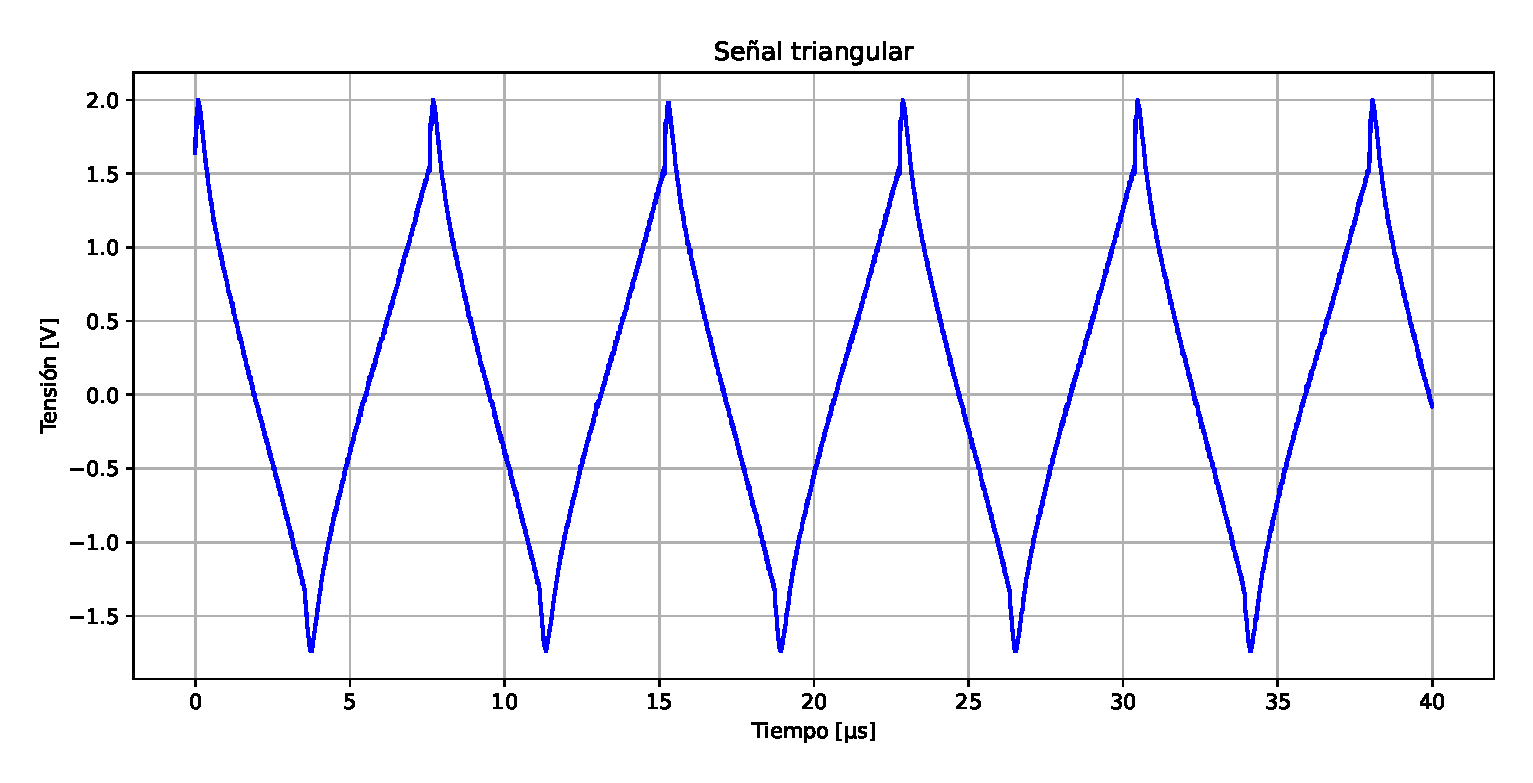
\includegraphics[width=\linewidth]{res/senal_triangular.eps}
    \caption{Señal triangular}
    \label{fig:señal_triangular}
\end{figure}
%%%%%%%%%%%%%%%%%%%%%%%%%%%%%%%%%%%%%%%%%%%%%%%%%%%%%%%%%%%
\section{Conclusiones}
\quad A lo largo del desarrollo se abordó el diseño y simulación de una fuente conmutada tipo Buck, donde se debió trabajar el control por modulación de ancho de pulso y el diseño físico del inductor. Durante la simulación, se observo que esta fuente Buck cumplió los requerimientos, superando el 90\% de eficiencia en distintas condiciones de carga, manteniendo a su vez un tiempo de establecimiento y un ripple acorde. 

\quad Se puso en práctica el diseño de pistas para circuitos de frecuencia, en donde se tuvo que considerar el trazado de pistas y el plano de masa. 
El diseño del circuito PWM se implementó mediante comparadores, logrando generar, luego de varios intentos, una señal triangular estable y una señal PWM capaz de controlar los MOSFETs.
%%%%%%%%%%%%%%%%%%%%%%%%%%%%%%%%%%%%%%%%%%%%%%%%%%%%%%%%%%%
\section{Apéndice}
%%%%%%%%%%%%%%%%%%%%%%%%%%%%%%%%%%%%%%%%%%%%%%%%%%%%%%%%%%%
\subsection{Calculo del inductor}

\quad Se utilizaron las siguientes especificaciones para realizar los cálculos:
\begin{center}
\begin{equation*}
\begin{aligned}
L &= \SI{300}{\micro\henry} \\
I_{L,max} &= \SI{1.54}{\ampere} \\
I_{L,dc} &= \SI{1.48}{\ampere} \\
f_{sw} &= \SI{130}{\kilo\hertz} \\
P_{cu} &= \SI{1}{\watt} \\
K_u &= 0{,}33 \\
\rho_{cu} &= \SI{1.7e-6}{\ohm\centi\metre}
\end{aligned}
\end{equation*}
\end{center}
\quad El campo magnético máximo se obtuvo de la hoja de datos del material observando el máximo valor donde la permeabilidad tiene un comportamiento lineal.Luego, los valores de corriente máxima y media fueron obtenidos cuando la carga es mínima $R_{L_{min}} = \frac{9V}{1.5A} = 6.33\ohm$

\quad El método \textit{Tacca} indica que en primer lugar se debe calcular la sección de hierro, $S_{fe}$.
\begin{center}
\begin{equation*}
\begin{aligned}
F_b &= K_u \\
F_v &= 0.25 \\
I_{L,ef} &= I_{L,dc} \\
\sigma_{IL} &= \SI{5}{ \frac{\ampere}{\milli\metre^2}}
\end{aligned}
\end{equation*}
\end{center}

\begin{equation}
    S_{fe} = 10\sqrt{\frac{LI_{L,ef}I_{L,max}}{F_bF_vB_{max}\sigma_{IL}}} = 0.744 cm^2 
\end{equation}
\quad Verificando la tabla provista por \textit{Ericksson} y la disponiblidad comercial, se decidio usar el nucleo \textit{EE3007}. Una vez decidido el nucleo es necesario verificar el valor del facotr de ventana, $F_v$, elegido. Para eso se utilizo la datasheet del nucleo para obtener las dimensiones de la pieza.
\begin{center}
    \begin{equation*}
        \begin{aligned}
            B &= \SI{19,6}{\milli\metre} \\
            C &= \SI{9,5}{\milli\metre} \\
            D &= \SI{6,5}{\milli\metre} \\
            E &= \SI{6,3}{\milli\metre} \\
            F &= \SI{6,3}{\milli\metre} \\
        \end{aligned}
    \end{equation*}
\end{center}
\begin{equation}
    F_v = \frac{S_v}{S_{fe}} = \frac{E(B-C)}{2CD} = 0.35
\end{equation}
\quad Considerando este valor se volvió a calcular la sección del hierro, $S_{fe} =\SI{0.629}{\centi\metre^2}$. La variación es pequeña por lo que la elección del nucleo continua cumpliendo. 

\quad Se procedió a calcular el valor del entrehierro. 
\begin{equation}
    12 \frac{L}{S_{fe}}(\frac{I_{L,max}}{B_{max}})^2 =\SI{0.151}{\milli\metre} 
\end{equation}

\quad Obtenido este valor, se pudo conseguir el numero de vueltas necesarias para el inductor. 
\begin{equation}
    n = 850\frac{B_{max}}{I_{L,max}}I_g = 25
\end{equation}

\begin{center}
    \begin{equation*}
        \begin{aligned}
            W_a = \SI{0.476}{\centi\metre^2}
        \end{aligned}
    \end{equation*}
\end{center}
\begin{equation}
    A_w \leq\frac{K_uW_a}{n} = \SI{6.283e-3}{\centi\metre^2}
\end{equation}
\quad Se elige usar el camble AWG\#20 que tiene un $A_w = \SI{5.188e-3}{\centi\metre^2}$. Se verifica que el valor de la densidad sea menor a \SI{5}{\frac{\ampere}{\milli\metre^2}} y que no sature
\begin{center}
\begin{equation*}
\begin{aligned}
    \sigma_{IL} = \frac{I_{L,max}}{100A_w} = \SI{2.789}{\frac{\ampere}{\milli\metre^2}} \\
    B_{max,real} = \frac{\mu_0nI_{L,max}}{I_g} = \SI{0.0003}{T}
\end{aligned}
\end{equation*}
\end{center}

\quad Finalmente, se verifico que no haya efecto pelicular, es decir que $\delta\leq r_{Cu}$. 
\begin{center}
\begin{equation*}
\begin{aligned}
    r_{Cu} =\SI{0.0437}{\centi\metre}\\
    \delta = \frac{7.5}{\sqrt{f_{sw}}} = 0.021
\end{aligned}
\end{equation*}
\end{center}





\end{document}